% =====================================================================
% VERSION ENSAE, REDUCTION SFE (phase 3, 1er octobre 2026) : chapitre 3, donnees.
% Copie a texte constant de chapitres/05_donnees_limites.tex.
% Ne changent que les titres et les renvois repares, listes dans
% reduction/phase3.md.
% Lu par main_ensae.tex seul : ne jamais le faire lire par main_institut.tex,
% qui garde chapitres/.
% =====================================================================

\chapter{Données}
\label{chap:donnees}
\label{part:donnees}

% MIGRÉ AUTOMATIQUEMENT depuis memoire/main.tex (plages 1002-1433).
% Hiérarchie descendue d'un cran, labels préfixés "don:".
% RELECTURE FAITE (août 2026). Aucune phrase du chapitre n'annonce la copule ni
% la variable latente comme LE modèle. Ajouts d'août : la table des trois
% fréquences, le seuil de collecte, et la section des deux biais chiffrés
% (élasticité de taille corrigée par troncature, chain-ladder de remontée).
%==============================================================

Trois bases alimentent le modèle, chacune pour la composante qu'elle peut renseigner.

%--------------------------------------------------------------
%--------------------------------------------------------------
\section{Sources et rôles}
\label{sec:carto}
%--------------------------------------------------------------

\begin{center}
\renewcommand{\arraystretch}{1.3}
\begin{tabular}{>{\raggedright}p{2.75cm} >{\raggedright}p{2.6cm} >{\raggedright}p{3.9cm} >{\raggedright\arraybackslash}p{4.05cm}}
\toprule
\rowcolor{lightblue}
\textbf{Source} & \textbf{Effectif retenu} & \textbf{Rôle dans le modèle} & \textbf{Justification / limite} \\
\midrule
PRC 2025 & $15\,053$ incidents, 2019 à 2025 & Sévérité alternative via conversion Jacobs ; nombre annuel de notifications $\lambda_{ref}$, décrit et non utilisé par le moteur &
Périmètre défini, mais sévérité dérivée d'un modèle log-log \\
\addlinespace
SAS OpRisk Global & $41\,975$ pertes, dont $582$ en cyber $\times$ finance, 1979 à 2026 & Sévérité (montants réels) et nombre annuel d'incidents du moteur ($\lambda$) &
Montants observés, mais biais vers les grandes entités financières \\
\addlinespace
Hackmageddon & $1\,041$ incidents, premier semestre 2026 & Parts par vecteur d'attaque (structure du risque) &
Ne fixe aucun niveau : pondère le multiplicateur qui fait passer $\lambda$ d'un état de conformité à l'autre \\
\bottomrule
\end{tabular}
\end{center}

Les articles~19 et~231 du règlement délégué (UE) 2015/35 exigent des données exactes, exhaustives et
appropriées, pour les provisions techniques et pour un modèle interne ; nous prenons ces critères pour référence. Aucune des bases que nous avons examinées ne remplit ces trois exigences. Nous documentons les biais de chaque source et leurs retraitements.

% SOURCES-SCRIPTS: 63 104

\section{Biais statistiques des sources}
\label{sec:trois-biais}

Trois biais affectent les bases PRC et OpRisk. Le
\emph{biais de sélection} touche OpRisk, qui recense surtout des pertes rendues publiques, donc
celles des grandes entités ou des montants exceptionnels. Il surreprésente les événements extrêmes,
et nous ramenons la fréquence et la sévérité à la taille de l'entité par deux élasticités estimées
(\S\ref{sec:biais-chiffres} et chapitre~\ref{chap:resultats}). Le \emph{biais de déclaration}
touche la PRC, car la notification des fuites de données personnelles est obligatoire dans la plupart
des États américains, pas celle d'un rançongiciel qui n'exfiltre rien. Le niveau de fréquence est
donc lu sur OpRisk, et la répartition par vecteur sur Hackmageddon.

Un \emph{biais de survie} pourrait sous-représenter les entités disparues, mais les pertes qui ont conduit à une faillite sont souvent publiques : ni son existence ni son signe ne sont établis sur ces bases, et il ne figure pas parmi les écarts mesurés du chapitre~\ref{ch:robustesse}.

\section{Hétérogénéité temporelle et actualisation des sinistres}

Le sous-échantillon cyber-finance OpRisk contient des pertes de $1979$ à $2026$, période sur laquelle les montants nominaux dérivent.
Pour chaque perte, la base donne le montant de l'année de l'événement et sa valeur courante, corrigée
de l'inflation générale. Leur rapport, égal à un pour les années récentes, atteint $1{,}747$ en
$2004$, d'où une inflation implicite de $2{,}19\,\%$ par an. Nous calibrons cependant sur le premier,
c'est-à-dire sur des montants \emph{nominaux}. Ce choix minore les sinistres anciens ramenés en euros
courants, donc la queue et le capital. Son effet sur la dérive des pertes est mesuré au
\S\ref{soc:sec:backtest}.
% SOURCES-SCRIPTS: 102

La PRC fournit la fréquence de référence $\lambda_{ref}$, qui compte des notifications sans seuil de
matérialité et ne fixe pas le niveau du capital. Elle sert aussi de source de sévérité indirecte : la conversion de \citet{jacobs2014}, $\ln(L) = 7{,}68 + 0{,}76\,\ln(X)$, donne la perte $L$ en dollars d'un incident à partir de son nombre $X$ d'enregistrements. Calibrée sur les $15\,053$ incidents 2019--2025 dont le volume touché est renseigné (la figure~\ref{fig:composition-temporelle-rapport} compte toutes les notifications), la queue PRC a un paramètre de forme $\hat{\xi}_{\text{PRC}} = 1{,}03$ (intervalle à $90\,\%$ :
$[0{,}97~;~1{,}09]$). À cette valeur, l'espérance est infinie. On ne la lit qu'avec le plafond de sévérité
propre à cette source \matcomp.

\begin{figure}[H]
\centering
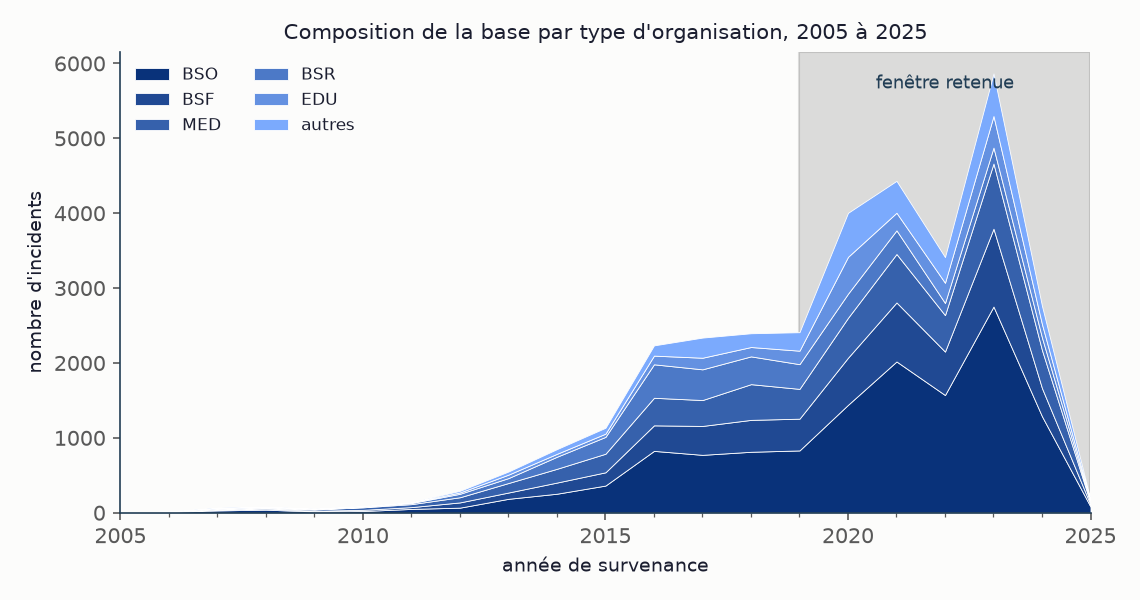
\includegraphics[width=0.78\textwidth]{D4_composition_temporelle.png}
\caption{Composition de la chronologie PRC par type d'organisation et par année. La zone grisée est
la fenêtre retenue. La hausse d'avant $2019$ suit l'extension de la collecte. La baisse de $2025$ traduit le manque de recul. BSF : organisations financières ; les autres codes sont ceux de la base.}
% SOURCES-SCRIPTS: 104
\label{fig:composition-temporelle-rapport}
\end{figure}



% SOURCES-SCRIPTS: 57 62 63

\section{Fréquences et seuils de collecte}

% SOURCES-SCRIPTS: 08b 60 62

La valeur de la fréquence dépend du périmètre de comptage de la source. Sur le
panel firme-année du SAS OpRisk (sous-catégories TIC, 2005--2022), le taux est de $0{,}10$ événement
par firme et par an toutes firmes confondues, et $0{,}21$ pour les firmes à au moins dix événements.
Au chapitre~\ref{chap:resultats}, nous estimons $\lambda$ comme une fonction de la taille de firme afin
de le lire à celle de l'entité notionnelle, ce qui donne $0{,}092$. Ces taux sont par firme ; celui du moteur compte le périmètre financier étudié. Le panel d'entité retient cinq sous-catégories TIC, plus larges que le filtre cyber-finance de sévérité : leur réconciliation reste nécessaire. Tous ne retiennent que les pertes au-dessus du seuil de collecte d'OpRisk. Ils comptent
donc les incidents TIC \emph{matériels}, pas tous les incidents au sens du reporting DORA.

Le taux par firme est une propriété d'entité, lisible sur un panel. Le tableau~\ref{tab:echelle} traduit ces échelles en capital.

Le terme de fréquence recouvre trois taux, à trois niveaux d'observation :
\begin{center}\small
\renewcommand{\arraystretch}{1.3}
\begin{tabular}{@{}l l r p{5.1cm}@{}}
\toprule
\textbf{Symbole} & \textbf{Source} & \textbf{Valeur} & \textbf{Ce qu'il compte} \\
\midrule
$\lambda_{ref}$ & PRC & $341$/an & notifications de violation de données des
\emph{organisations financières} de la base PRC (code \texttt{BSF}), et non de la base
entière, qui en compte $2\,150$ par an. Décomposée par vecteur d'attaque ; n'entre pas dans le moteur et ne fixe aucun niveau de capital. \\
$\lambda$ & OpRisk & $21{,}6$/an & incidents TIC \emph{matériels} du secteur
financier mondial. C'est l'entrée du moteur de cascade et le seul des trois dont dépend le capital. \\
$\lambda_{\text{entité}}$ & OpRisk & $0{,}092$/an & les événements TIC du panel, rapportés
à \emph{une} firme et lus \emph{à la taille} de l'entité notionnelle. C'est
l'échelle de lecture d'une entité soumise à DORA. \\
\bottomrule
\end{tabular}
\end{center}
Le facteur $3\,719$ entre $\lambda_{ref}$ et $\lambda_{\text{entité}}$ sépare trois comptages, ceux des notifications, des pertes
matérielles du secteur et des pertes matérielles par entité. Le moteur de simulation n'utilise que
$\lambda$.
% SOURCES-SCRIPTS: 67

\section{Effet chiffré de deux biais}
\label{sec:biais-chiffres}
% SOURCES-SCRIPTS: 57

Corrigée de la troncature au seuil de collecte, l'élasticité de la sévérité à la taille est de
$b=0{,}087$, et la sévérité transposée à l'entité notionnelle n'est multipliée que par $0{,}861$. Le
biais de taille est réel, mais faible. On corrige la troncature à droite par chain-ladder : les $97$ événements observés sur 2023--2025 deviennent $255$ à l'ultime, soit $85{,}0$ par an contre $74{,}1$ sur 2015--2022, et la fréquence est relevée d'un facteur $1{,}147$. Le risque TIC n'a donc pas
baissé après 2022, il n'est pas encore remonté dans la base. Les régressions et le triangle de
développement sont déportés \matcomp.
% SOURCES-SCRIPTS: 67

Les deux corrections se compensent presque sur la perte moyenne, $0{,}861\times1{,}147=0{,}987$, soit
un effet net de $1{,}3\,\%$, inférieur à l'incertitude d'estimation de chacune, mais elles ne se compensent pas sur le capital. À queue lourde, le quantile à $99{,}5\,\%$ répond à la sévérité bien plus qu'à la fréquence. Leur effet net sur le capital n'est pas chiffré. La correction de taille agit sur la sévérité et celle de troncature sur la fréquence ; leur compensation sur la moyenne ne détermine pas le signe de l'effet sur le quantile.

\section{Hackmageddon et la structure du risque}
\label{sec:hackmageddon}

Hackmageddon donne la \emph{structure} du risque, jamais son niveau. Le décompte retenu couvre le
semestre janvier--juin 2026, avec 1\,041 incidents, dont 840 à vecteur d'accès initial identifié
($81\,\%$). Le jeu consulté n'a pas été conservé ; relu en octobre 2026 avec une autre grille, il ne redonne pas ces décomptes à l'unité. Ce sont des citations datées. Ils fixent les parts de répartition par vecteur, qui pondèrent le
multiplicateur de fréquence entre états de conformité (\S\ref{sec:quatre-canaux}). Ce
multiplicateur hérite donc de leur statut de citation.

\begin{center}
\renewcommand{\arraystretch}{1.3}
\begin{tabular}{>{\raggedright}p{5cm} c >{\raggedright\arraybackslash}p{6cm}}
\toprule
\rowcolor{lightblue}
\textbf{Vecteur d'attaque} & \textbf{Part} & \textbf{Exigence DORA} \\
\midrule
Hameçonnage / ingénierie sociale & $38{,}8\,\%$ & Art.~13, sensibilisation \& formation \\
Exploitation vuln.\ exposée & $33{,}8\,\%$ & Art.~26, tests TLPT ; Art.~8--10 \\
Chaîne d'approvisionnement / tiers TIC & $15{,}8\,\%$ & Art.~28--44, gestion du risque tiers \\
Identifiants compromis & $6{,}3\,\%$ & Art.~9, contrôle d'accès \& MFA \\
\bottomrule
\end{tabular}
\end{center}

Deux parts structurent les scénarios du chapitre~\ref{chap:multietats} : $15{,}8\,\%$ des attaques
empruntent le vecteur tiers, objet des articles~28 à~44, et $49{,}6\,\%$ (dont ces $15{,}8\,\%$) relèvent de vecteurs qu'un
test TLPT est censé détecter en amont. La base recense des incidents rendus publics, ce qui interdit
d'en tirer un niveau de fréquence, et sa taxonomie est instable. La catégorie rançongiciel n'existait
pas en 2023, et une lecture naïve lui prête une hausse de 11 points là où, après reclassement, elle recule de 23 points. Seules les motivations se comparent directement dans le temps. Les catégories bâloises de la base SAS informent trop faiblement la sévérité pour fonder une segmentation (\S\ref{sec:profilage-variables}).

% SOURCES-SCRIPTS: 63

\section{OpRisk Global et la sévérité en euros}
\label{sec:oprisk}

% SOURCES-SCRIPTS: 07 47 63

OpRisk Global est la base de référence historique du risque opérationnel au sens de Bâle. Le risque cyber y est reconstruit à
partir des catégories \og Systems Security\fg{} et \og Business Disruption and System Failures\fg{}, et
le périmètre cyber $\times$ finance compte 582 incidents, dont certains sont antérieurs à 2000. Le dénominateur de 27 ans utilisé pour la fréquence est une convention de calibration ; il ne correspond pas à toute la période observée. Une recalibration cohérente du filtre temporel et de la fréquence reste nécessaire. \citet{elingwirfs2019}
en extraient également les pertes d'origine informatique. Cette base alimentait les modèles internes de
mesure avancée (section~\ref{chap:reglementaire}), qui calibraient la sévérité extrême sur des pertes
observées sans passer par un indicateur de volume. Nous reprenons cette logique.

Sur la population de la fréquence (secteur financier, catégories TIC, 2005--2022, $1\,476$
observations), la sévérité se décrit ainsi :
\begin{center}
\renewcommand{\arraystretch}{1.3}
\begin{tabular}{l r l r}
\toprule
\rowcolor{lightblue}
\textbf{Indicateur} & \textbf{Valeur} & \textbf{Indicateur} & \textbf{Valeur} \\
\midrule
Médiane & 1{,}20 M\$ & P99 & 419{,}3 M\$ \\
Moyenne & 33{,}8 M\$ & Maximum & 10\,970{,}8 M\$ \\
P90 & 25{,}3 M\$ & Total cumulé & 49{,}8 Md\$ \\
\bottomrule
\end{tabular}
\end{center}
Les montants de ce tableau sont en dollars ; le moteur les convertit en euros au taux fixe de $0{,}92$. Le décile supérieur concentre $92{,}3\,\%$ de la perte totale et le centile supérieur $65{,}1\,\%$,
ce qui justifie la théorie des valeurs extrêmes du chapitre~\ref{chap:socle}.
% SOURCES-SCRIPTS: 67

Nous ajustons la loi de Pareto généralisée sur les $582$ pertes cyber $\times$ finance au-delà d'un
seuil $u = 20$~M\euro, proche du percentile~85 des montants, où le graphique des excès moyens devient
linéaire (figure au supplément, \S\ref{don:fig:mep}). Avec $91$ excès, on obtient :
\[
\hat{\xi} = 0{,}595 \quad (\text{IC}_{90\%}=[0{,}30\,;\,0{,}83]), \qquad
\hat{\sigma} = 58{,}0~\text{M\euro}, \qquad
\qsev_{99{,}5\%}(X) = 663~\text{M\euro}.
\]
Le dernier terme est le quantile de la sévérité d'un sinistre, pas un capital, car le besoin de capital
est le quantile de la charge annuelle agrégée, obtenu par composition avec la fréquence. L'intervalle
bootstrap de ce quantile, $[411\,;\,1037]$~M\euro, couvre un facteur~2{,}5. L'écart avec la PRC
($\hat{\xi}_{\text{PRC}} = 1{,}03$) ne mesure pas une différence de risque : la sévérité PRC
est une puissance de pente $0{,}76$ du nombre d'enregistrements, et une puissance multiplie l'indice
de queue par son exposant. Les deux indices sont positifs ($\xi > 0$), sur deux objets différents.

%--------------------------------------------------------------
\section{Analyse exploratoire et profilage des variables}
\label{sec:profilage-variables}
%--------------------------------------------------------------
% SOURCES-SCRIPTS: 104

Le profilage des variables des deux bases, détaillé dans le supplément, montre d'abord que, dans la
chronologie PRC, un champ non renseigné prend la valeur \texttt{UNKN} au lieu d'être vide. Le nombre d'enregistrements touchés n'est ainsi documenté que dans $41{,}77\,\%$ des cas. De plus, la base n'agrège pas les
notifications, si bien qu'un même incident déclaré à plusieurs autorités y figure plusieurs fois. La
déduplication retire $1\,643$ lignes, soit $10{,}9\,\%$ des lignes, une borne basse. Nous n'additionnons jamais ces volumes, mais les doublons pèsent encore sur les comptages et sur l'ajustement de la sévérité ; leur effet n'est pas chiffré.

La chronologie PRC compte $74\,783$ incidents, dont $31\,217$ documentent un volume touché
positif. La base SAS compte $41\,976$ lignes brutes et $41\,975$ pertes après retrait d'une
aberration de saisie, dont $1\,099$ en catégories TIC et $582$ dans le croisement cyber $\times$
finance retenu pour la sévérité. Le tableau donne pour chaque variable son type, son rôle et la part
de lignes renseignées, \texttt{UNKN} compté comme un manquant.

\begin{center}\footnotesize
\renewcommand{\arraystretch}{1.05}
\begin{tabular}{@{}>{\ttfamily\raggedright}p{3.35cm} l >{\raggedright}p{5.1cm} l r@{}}
\toprule
\textbf{Variable} & \textbf{Type} & \textbf{Rôle dans le modèle} & \textbf{Base} & \textbf{Renseignée} \\
\midrule
total\_affected & quantitative & enregistrements touchés, seule mesure d'impact de la base & PRC & $41{,}77\,\%$ \\
residents\_affected & quantitative & sous-ensemble territorialisé du précédent & PRC & $79{,}88\,\%$ \\
breach\_date & temporelle & date de survenance, support de la fréquence annuelle & PRC & $54{,}82\,\%$ \\
reported\_date & temporelle & date de notification, support du délai de détection & PRC & $99{,}54\,\%$ \\
end\_breach\_date & temporelle & fin d'exposition, support de la durée d'incident & PRC & $28{,}18\,\%$ \\
organization\_type & qualitative & classe d'organisation, huit modalités & PRC & $89{,}29\,\%$ \\
breach\_type & qualitative & vecteur de la brèche, huit modalités & PRC & $47{,}31\,\%$ \\
\midrule
Loss Amount & quantitative & montant de perte avérée, source de la sévérité & SAS & $100\,\%$ \\
Event Risk Category & qualitative & catégorie bâloise de niveau 1, sept modalités & SAS & $100\,\%$ \\
Sub Risk Category & qualitative & sous-catégorie, définit le périmètre TIC & SAS & $100\,\%$ \\
Basel Business Line & qualitative & ligne métier, dix modalités & SAS & $100\,\%$ \\
Industry Sector Name & qualitative & secteur, définit le périmètre financier & SAS & $100\,\%$ \\
Revenue & quantitative & chiffre d'affaires, mesure de taille & SAS & $87{,}82\,\%$ \\
Assets & quantitative & actif total, mesure de taille prudentielle & SAS & $83{,}51\,\%$ \\
\bottomrule
\end{tabular}
\end{center}

Le volume touché est la variable d'impact la moins bien renseignée, et pas au hasard : les champs
qu'impose l'obligation de notification sont remplis, ceux qui demandent une enquête ne le sont pas.
Le manquant est donc plausiblement corrélé à la gravité, ce qui explique que le modèle ne conditionne
la sévérité sur aucune de ces variables.

La perte n'est ni normale ni log-normale. Après passage au logarithme, le test de Shapiro-Wilk rejette encore la normalité (statistique $W=0{,}970$ sur les enregistrements PRC, $W=0{,}986$ sur les pertes SAS). Nous modélisons donc la seule queue, par une loi de Pareto généralisée au-delà d'un seuil.

Sur $33\,769$ pertes à profil financier complet, le $V$ de Cramér reste sous $0{,}20$,
l'$\varepsilon^2$ de Kruskal-Wallis sous $0{,}08$, et les corrélations de rang entre perte et taille
sous $0{,}16$. Ces tailles d'effet sont faibles, et nous ajustons une queue commune. C'est une hypothèse : l'indice varie selon la catégorie bâloise, et aucune base n'observe la sévérité par pilier. L'actif
total est le moins lié à la perte des trois mesures de taille ($0{,}068$, contre $0{,}159$ pour le
chiffre d'affaires et $0{,}139$ pour l'effectif). La mise à l'échelle du chapitre~\ref{chap:resultats} utilise pourtant le bilan, le prédicteur le plus faible des trois ; c'est une hypothèse du modèle.

\section{Limites des données}
\label{sec:portee-donnees}

Les pertes observées donnent une fréquence d'incidents, modulée entre états de conformité selon la répartition des attaques citée. Elles servent aussi à calibrer une
sévérité de queue lourde sur OpRisk, à la confronter à une source indépendante et à traiter l'écart
entre sources comme une incertitude à part entière.

Ces données ne mesurent pas la conformité DORA d'une entité ; nous posons donc l'état de chaque pilier (chapitre~\ref{chap:multietats}). Il
n'existe pas de base d'incidents harmonisée, exhaustive et exempte de biais de visibilité. Faute
d'historique d'événements joints, on ne peut pas estimer la corrélation entre les pertes des piliers, que
nous traitons au chapitre~\ref{chap:cascade} par une structure de dépendance explicite. Le registre des incidents majeurs que DORA instaure atténuera ces limites sans les lever : limité aux incidents au-dessus d'un seuil de matérialité, il restera tronqué.

S'il renseigne la taille de l'entité et le prestataire en cause, il permettra de conditionner la sévérité à la taille et cartographiera les prestataires tiers ; l'effet d'une telle donnée sur le capital est chiffré au chapitre~\ref{chap:partielle}. Le modèle ne dépend pas de la source : substituer ce registre aux bases PRC et OpRisk ne change pas sa structure.

% SOURCES-SCRIPTS: 05 63

\section{Nombre de sources retenues}

D'autres bases existent, sinistres cyber assurantiels ou enquêtes sectorielles, mais chacune
comporterait ses propres biais et ne comblerait pas l'absence d'un registre harmonisé. Dans l'analyse de sensibilité du chapitre~\ref{chap:resultats}, l'incertitude sur l'indice de queue de la sévérité domine toute autre source de variation du modèle. Une base de plus ne la réduirait que si elle apportait des pertes en montant au-delà du seuil. Les parts par vecteur tirées de
Hackmageddon sont du même ordre dans le rapport \emph{ENISA Threat Landscape 2025} \citep{enisa2025}, collecté autrement \matcomp.

Les données fixent la queue de sévérité ($\hat\xi = 0{,}595$ sur OpRisk) et le nombre annuel d'incidents $\lambda$. L'accumulation chez un prestataire commun est posée, et la direction de la contagion n'est pas identifiée (chapitre~\ref{ch:identifiabilite}), d'où les bornes de capital du chapitre~\ref{chap:partielle}.

% SOURCES-SCRIPTS: 05 62 63
